\documentclass{tufte-book}

\usepackage[utf8]{inputenc} % uft8?
\usepackage[T1]{fontenc}

\usepackage{graphicx}

\usepackage{color}
\usepackage{xcolor}
\usepackage{framed}
\usepackage{listings}

\usepackage[normalem]{ulem}

\usepackage{multicol}              
\usepackage{multirow}
\usepackage{booktabs} 

\usepackage[innerrightmargin = 0.7cm, innerleftmargin = 0.3cm]{mdframed}
\usepackage{mdwlist}

\usepackage{morefloats} % to take care of too many floats caused by the marginnotes

\usepackage[]{hyperref}
\definecolor{darkblue}{rgb}{0,0,.5}
\hypersetup{colorlinks=true, breaklinks=true, linkcolor=darkblue, menucolor=darkblue, urlcolor=darkblue, citecolor=darkblue}


\setcounter{secnumdepth}{1}
\setcounter{tocdepth}{1}


\title{Research skills\\
\large{An introduction to the crafts of a scientist}}
\author{Florian Hartig, University of Freiburg}

\begin{document}
\let\cleardoublepage\clearpage
\maketitle


\thispagestyle{empty}
\null

\begin{fullwidth}
This script is part of the course material for the MSc model Research Skills, University of Freiburg (website \href{http://florianhartig.github.io/ResearchSkills/}{here}). First edition 2015, created \today.\\[0.5cm]
\end{fullwidth}

\href{https://florianhartig.wordpress.com/}{Florian Hartig}\\
University of Freiburg\\
Germany\\[0.2cm]
If you find typos or have suggestions, please report them by creating a ticket \href{https://github.com/florianhartig/ResearchSkills/issues}{here}




\paragraph{Acknowledgments:}Severin Hauenstein for contributions to the chapter on scientific writing.


\vfill
\begin{fullwidth}
This work is licensed under a Creative Commons Attribution-NonCommercial-NoDerivatives 4.0 International License.
\end{fullwidth}


\newpage
\tableofcontents

\newpage




\chapter{Logic and philosophy of science}

\section{What is science?}

The Oxford dictionary defines science as 

\begin{quote}
Science [mass noun] - the intellectual and practical activity encompassing the systematic study of the structure and behavior of the physical and natural world through observation and experiment.
\end{quote}

\noindent Or, in the words of Richard Feynman:

\begin{quote}
Science is a process for learning about nature in which competing ideas about how the world works are measured against observation.
\end{quote}

Hence, science is a method to find out how the natural world world works based on observations. The latter distinguishes the sciences from the arts (e.g. paintings, music, dance), and from the humanities that study aspects of human culture (e.g. languages, literature, philosophy and history). The distinction between humanities and sciences has become less clear, however, because fields such as linguistics, economics or sociology are increasingly using the same formal approaches as the natural sciences. For these fields, the terms social sciences are now commonly used. 

The increasing adaptation of scientific methods also in disciplines that are not classically counted to the sciences has good reasons. In the last centuries, the scientific method has been the reason for an unprecedented increase in knowledge, opportunity and human well-being. As a result, science has become the most widely accepted answer to what one can know and how to find it out (epistemology), at least in the western world. 

\marginnote{Epistemology, from Greek episteme = knowledge and logos = word is the branch of philosophy concerned with what knowledge is, how it can be acquired, and what can be known}

But science is also a human endeavor. ``Science" may as well refer to the history of science, the state of scientific knowledge, or science as a social institution. Those latter aspects of science are less formally defined and stable that science as a method - if we look at the history of science, we see individuals that are unified by a common cause, but that are at the same time subject to their national and cultural influences as well as by personal vanity, pride or madness.\marginnote{Many famous scientists engaged in personal and irrational feuds. For example, the doubtlessly ingenious Isaac Newton engaged in countless spiteful and bitter fights, including his most famous battle with German mathematician Gottfried Leibniz over the invention of infinitesimal calculus.} As a result, the history of science, as well as its present state, is complicated by personal preferences, power games and random events, in the same way as political and economic history is. 

In the center of science, however, remains a set of assumptions and methods, a philosophy if you will, that allows us to draw and agree on conclusions from empirical observations. Not every scientist is aware of the ``formal rules" of these methods, but that does not mean that (s)he would not apply them. In his book "Induction \& Intuition in Scientific Thought", Peter Medawar notes: 

\begin{quote}
The fact that scientists do not consciously practice a formal methodology is very poor evidence that no such methodology exists. It could be said—has been said—that there is a distinctive methodology of science which scientists practice unwittingly, like the chap in Molière who found that all his life, unknowingly, he had been speaking prose.
\end{quote}

It may thus be possible to do science without having ever learned the basics of the scientific method. However, that does not mean you should not learn about the methods of science. An amateur can sometimes do great work, from intuition and practice, but without a good education s(he) may fail in other situations. Learning the rules of science will provide you with saveguards against drawing false conclusion, will teach you methods to make discovery and communication more efficient, and will arguable improve your general understanding of the world. Hence, read this manual for science with care, including the  rest of this chapter, which is devoted to laying out the assumptions and history of science, and discussing how the "scientific method" works. 


\section{Philosophical foundations of scientific thinking}



\subsection{Logic}

Logic\marginnote{Statements or claims that can be true or false are called propositions. If we use propositions in an argument, we call them premises. The result of an argument is called a conclusion.} deals with the standards and criteria to evaluate the validity of reasoning. In classical education, it is a counterpart to rhetoric, which studies how to formulate arguments convincingly (even if they are not true). 

The study of logic is sometimes further subdivided into informal and formal logic. Informal logic evaluates the validity of arguments presented in ordinary language, while formal logic is concerned with the validity of arguments in formalized or mathematical language. There is no fundamental difference between the rules of logic in those two areas, but informal logic is presented with the additional challenge to examine the implicit premises (sometimes also called warrants) included in verbal arguments. 


\subsection{Empiricism and induction}

Empiricism\marginnote{Famous empiricists are, e.g., Hume or John Stuart Mill} is the stance that (scientific) knowledge comes only from observations. For an empiricist, (sensory) experience is more important for the formation of ideas about how the world works than logical reasoning or innate knowledge. 

\paragraph{Inductive reasoning}\marginnote{Induction = conclusion from the specific to the general} An important idea in the context of empiricism is the concept of inductive reasoning. An induction is a conclusion from particular instances to the general. Example: all swans I have seen are white, therefore all swans are white.\marginnote{Empiricism != induction} Empiricism does not prescribe the use of inductions for generating knowledge, but it seems obvious that pure empiricism would require to rely on inductive reasoning if any general conclusions are to be generated. 


\paragraph{The problem of induction}The problem\marginnote{Inductions are not always correct} with inductive reasoning is evident - an inductive conclusion does not need to be correct, even if the assumptions (observations, formal logic) are formally correct. Hence, we cannot be truly be sure if the knowledge that is created by empiricism and inductive reasoning is reliable. This problem has been named the ``problem of induction" by David Hume, but it was of course known for a long time. Sextus Empiricus (c. 160-210 AD), the name father of empiricism, observed famously:\marginnote{C. D. Broad remarked more shortly: ``Induction is the glory of science and the scandal of philosophy"}

\begin{quote}
When they propose to establish the universal from the particulars by means of induction, they will effect this by a review of either all or some of the particulars. But if they review some, the induction will be insecure, since some of the particulars omitted in the induction may contravene the universal; while if they are to review all, they will be toiling at the impossible, since the particulars are infinite and indefinite. Sextus Empiricus (c. 160-210 AD)
\end{quote}

Because of the problem of induction, there has always been a stain on inductive reasoning, and philosophers have tried to avoid relying on it for drawing conclusions about the world


\subsection{Rationalism and deductions}

\begin{figure}[]
\begin{center}
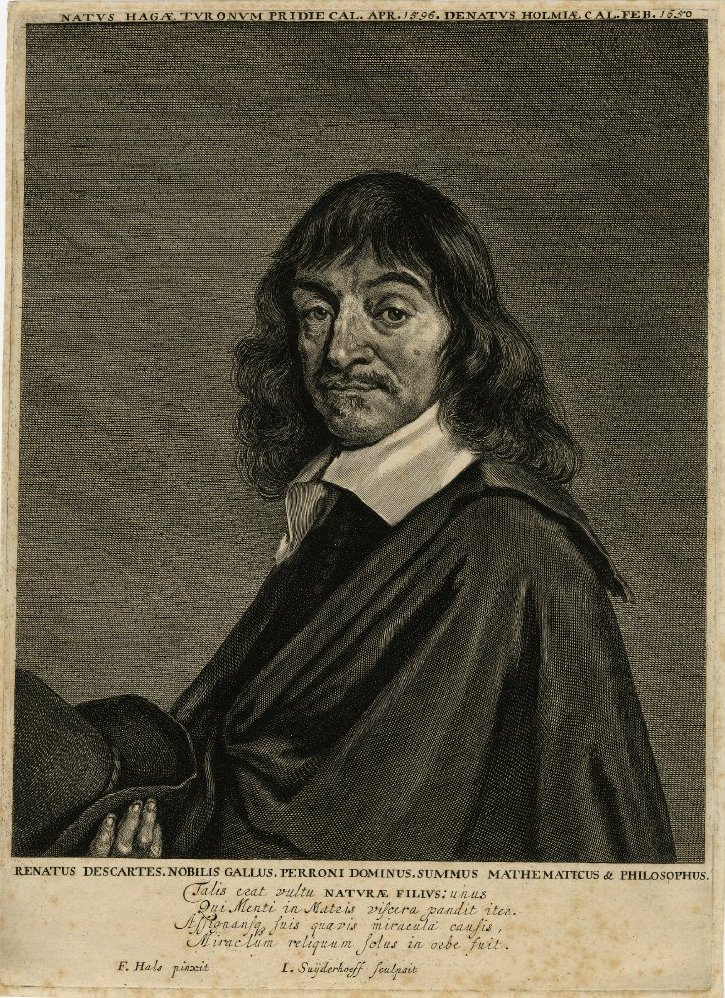
\includegraphics[width = 4cm]{figures/Descartes}
\caption{Portrait of René Descartes}
\label{fig: Descartes}
\end{center}
\end{figure}


Rationalism, in contrast to empiricism, holds the view that knowledge is created mainly by reasoning. In one of the foundational works of modern science, "Le Discours de la Méthode (1637)"  \footnote{The full title of this famous essay is "Discourse on the Method of Rightly Conducting One's Reason and of Seeking Truth" \citep{Descartes-DiscourseMethodRightly-1673}}, René Descartes famously observed: 

\begin{quote}
Good sense is\marginnote{ These words of one of the founding fathers of Science are often read as a sarcastic observation of human vanity. However, if one continues reading, it becomes clear that Descartes may, after all, have been serious about his faith in human rationality - he continues: ``And in this it is not likely that all are mistaken. The conviction is rather to be held as testifying that the power of judging [...] is by nature equal in all men; and that the diversity of our opinions, consequently, does not arise from some being endowed with a larger share of reason than others, but solely [because] we conduct our thoughts along different ways, and do not fix our attention on the same objects. ''}, of all things among men, the most equally distributed; for every one thinks himself so abundantly provided with it, that those even who are the most difficult to satisfy in everything else, do not usually desire a larger measure of this quality than they already possess.
\end{quote}

Pure thinking and logical conclusions are a fine thing, but a problem for a pure rationalist is that s(he) still needs something to think  about - from where do the objects and basic assumptions arise to which we can apply our rational thoughts? Rationalists differ though in their view on this matter. Some philosophers have stressed experience as providing these starting points, while others have maintained that there are some innate concepts or truths that we can know without reference to the material world. 

\paragraph{Deductive reasoning}Wherever\marginnote{Deductive reasoning = conclude from the general to the specific.} the starting points of rationalism come from, the reasoning natural to rationalism is deductive reasoning. A deduction is a conclusion from the general to the specific.\marginnote{In logic, the applewine example would be called a syllogism (Greek: syllogismos, "conclusion, inference" - a deductive argument based on two or more premises). The classical form, defined by Aristotle, consists of a general statement (the major premise) with a specific statement (the minor premise). In rhetoric, the major premise is often omitted, assuming the audience intuitively accepts it "Socrates is mortal because he is a human" - this is called an Enthymeme} 
See \href{https://en.wikipedia.org/wiki/Syllogism}{wikipedia} for further explanations. Example: all people from Frankfurt like applewine, I am from Frankfurt, therefore I like applewine. The last sentence 

An important difference to inductive reasoning is that, if assumptions are correct, conclusions made by deduction are necessarily correct. This is an important motivation for the further development of the scientific method.


\section{The basic science stance}

In the previous section, we have learned about two fundamentally different thoughts about how knowledge is created (empiricism and rationalism), and we have learned about two types of reasoning (induction and deduction). An attentive reader has probably already drawn a conclusion: in some way, science combines these two views. Before we come to that, however, let me define the basic assumptions that underlie the scientific method:\marginnote{You may find it trivial to make these statements, but even in academic circles, people often deny these assumptions in particular circumstances. For example: ``there are some things that you can simply not measure'', or ``not everything can be expressed in a formula''.}

\begin{itemize}
\item There is a material reality, and we can observe it.
\item The material reality follows certain general laws.\marginnote{Laws differ from scientific theories in that they do not propose a mechanism or explanation for the observed natural phenomena} We can discover the nature of these laws and their underlying causes (scientific theory), and we can do this objectively, meaning that everyone sharing the same basic principles (the scientific method) will agree eventually
\item Discovery happens by (a limited number of) empirical observations (empiricism) and reasoning (rationalism), which are combined in the scientific method. 
\end{itemize}

The\marginnote{There have been some fierce debates in the 90's between classical scientists and postmodernist. An example is the so-called Sokol affair, when the physics professor Alan Sokal published a nonsense-article full of deliberately incomprehensible jargon in a post-modernist academic journal in an attempt to expose the methodological weakness of this discipline \citep{Sokal-BeyondhoaxScience-2008}} first two statements express what is known in philosophy as positivism. Note that there are parts of social science (but not the natural sciences) that actively deny the truth of these statements. A notorious example are extreme positions of social constructionism and postmodernism, which broadly hold the view that reality and truth are not absolute, but constructed or negotiated through the interactions in a society.

% TODO add Postmodernism Generator, Fashionable Nonsense, higher superstition


\section{The scientific method and its history}\label{sec: scientific method}

\marginnote{A wider account of the different views on the scientific method on wikipedia \href{https://en.wikipedia.org/wiki/History_of_scientific_method}{here}}

By now, we have learned about rationalism and empiricism, and we have defined the basic assumptions of science, but we are yet to learn how we can bring these parts together to create scientific knowledge. Hence, we still have to discover the heart of science - the scientific method. 

\subsection{Aristotle's view on the scientific method in his Posterior Analytics}


One of the first\marginnote{Aristotle's six standard works on logic are summarized in the Organon. His view on the scientific method are spread around this work, but the main part is in the the ``Posterior Analytics'', (Latin: Analytica Posteriora).}, certainly one of the best-known explanations of the scientific method is Aristotle's inductive-deductive method (Fig.~\ref{fig: InductiveDeductiveAristotle}). The idea depicted in the figure is the following 

\begin{figure}[]
\begin{center}
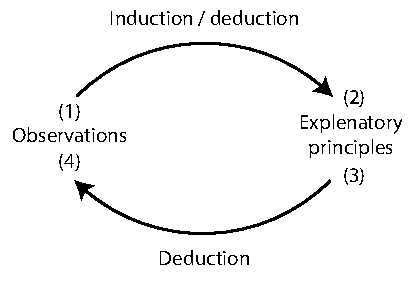
\includegraphics[width = 6cm]{figures/InductiveDeductiveAristotle.pdf}
\caption{Aristotles inductive-deductive model of the scientific method.}
\label{fig: InductiveDeductiveAristotle}
\end{center}
\end{figure}

\begin{enumerate}
\item You make an observation
\item Infer general principles from the observation
\item Infer consequences of these principles
\item Check them against observation
\item Potentially repeat
\end{enumerate}

This basic idea has not changed enormously in the next 2000 years, but it has changed in subtle details. Philosophers and scientists have developed different opinions about how the processes of generating explanatory principles and testing them works exactly. A particularly controversial topic has been the extent to which induction plays a role in this cycle. 

Aristotle suggests towards the end of the Posterior Analytics that, at first, explanatory principles arise through induction

\begin{quote}
    Thus it is clear that we must get to know the primary premises by induction; for the method by which even sense-perception implants the universal is inductive. 
\end{quote}

However, he is clearly uncomfortable with the inductive element in this and goes on to say that about the premises created by induction

\begin{quote}
[...] it follows that there will be no scientific knowledge of the primary premises, and since except intuition nothing can be truer than scientific knowledge, it will be intuition that apprehends the primary premises. 
\end{quote}

How this intuition works to create our first premises remains then a bit unclear - but you should read Aristotle yourself, maybe you can make more sense of it than me. 

\subsection{Popper and the scientific method}

We stay with the problem of induction, but take a 2000-yr leap to the the arguably most influential interpreter of the scientific method in the 20th century: Karl Popper\marginnote{Karl Raimund Popper (28 July 1902 – 17 September 1994), born into a Jewish middle-class family in Austria-Hungarian Vienna, is widely regarded as one of the most influential philosophers of the 20th century}. Popper developed the current orthodox interpretation of how science works. You may not like it, but the fact is that many, probably most scientists subscribe to his views as a basic description of the scientific method. Hence, don't act openly against it, and if people ask you how science works, the save bet is to recite Popper! 


\begin{figure}[]
\begin{center}
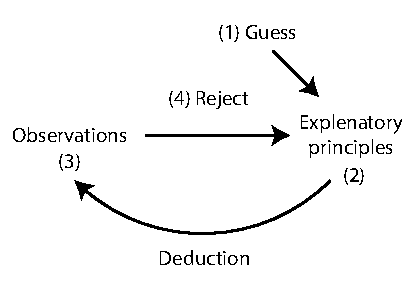
\includegraphics[width = 6cm]{figures/HypotheticoDeductivePopper.pdf}
\caption{Popper's hypothetico-deductive model of the scientific method}
\label{fig: InductiveDeductiveAristotle}
\end{center}
\end{figure}

\paragraph{Hypothetico-deductive method} One\marginnote{Popper developed the hypothetico-deductive interpretation of the scientific method, the currently accepted orthodox narrative of how science works} of Popper's main contributions to the scientific method was to take a radical step and remove the induction completely from the scientific equation. According to Popper, the essence of science is not to produce new theories, but to have a method to reject them. We don't care how new theories arise: they may be guessed, they may be induced, this is not part of the scientific method. The methods starts once we have a theory: we look at the predictions of this theory (deduction), we can test it against observation and see whether the theory is compatible with it (deduction), and if not, we can conclude that the theory is wrong (deduction). Through this construction, science consists only of logically clean deductions. Here a summary of this method - again, if someone asks you what the scientific method is, this is what you should say:

\marginnote{A hypothesis is a proposed law or explanation for a natural phenomenon.}

\begin{enumerate}
\item Form / guess a hypothesis about a scientific law or a theory that explains a phenomenon in nature
\item Derive predictions from this hypothesis
\item Test those predictions against observation
\item Draw conclusions about the validity of the hypothesis
\end{enumerate}

It\marginnote{You cannot prove a theory, you can only reject. Hence, never write: ``we proved A'' - if you must, write ``the data is compatible with A''} follows from Popper that ``you cannot prove a theory, you can only reject'' - hence, avoid using the word proof in scientific articles - many people care deeply about Popper, and they will react strongly to it! 


% TODO Yet, even Popper allows for "provisional truths" if 

% TODO working hypothesis

% TODO falsifiable - not even wrong \marginnote{A requirement for a scientifically valid hypothesis is that it is testable / falsifiable.}


\subsection{Multiple working hypothesis}

Popper is the mainstream, but there have been other suggestions about how science works or should work. A counterpoint to Popper's idea of rejection is the idea of multiple working hypothesis. The basic principle is simple - instead of trying to reject an idea, one can work with alternative theories. With time, evidence typically moving to favor one of them. \citet{Platt-StrongInferenceCertain-1964} tracks the history of this idea to an influential essay of the Geologist T. C. Chamberlin, who recommended working with multiple hypothesis to avoid as the best way to avoid “parental affection” (T. C. Chamberlin 1890, Science).

\subsection{Kuhn and variations of the scientific method}

The argument for multiple working hypothesis is a first example that includes social aspect of how science works into the method - the problem that Chamberlin has with the idea of Popper (he formulated his view before Popper of course) is not that Popper's method wouldn't work in principle, but that in practice, researchers may be hesitant to reject ideas, because they like them to be true. 

A more modern position that goes in a similar direction are the ideas of Thomas Kuhn\marginnote{Thomas Samuel Kuhn (July 18, 1922 – June 17, 1996) was an American physicist, historian, and philosopher of science.}: in his seminal work ``the structure of scientific revolutions'', Kuhn posits that sciences works within certain assumptions. In a normal science phase, we may apply Popper's idea to test and improve these assumptions, but we would not reject the basic premises even if there is evidence against them, unless a better theory emerges (revolutionary phase). The phases of science, according to Kuhn, are thus:

\begin{itemize}
\item Pre-paradigm phase – no consensus about a certain phenomenon, incomplete theories
\item Normal science – dominant paradigm emerged, progress in small steps within, but no questioning of paradigm, problems accumulate
\item Revolutionary science – paradigms redefined
\end{itemize}

There is probably a good deal of truth in this observation - in the history of science, there are many examples of the fact that an old theory is only rejected if a better theory is on offer. 

\section{Summary: the principles of science}

Bringing these different theories together, I think it's important not to interpret Aristotle, Popper, Chamberlin or Kuhn as opposing each other - I would simply say that they highlight different aspects of the scientific enterprise. 

Popper offers arguably the most pure account of a logically consistent way to use empirical arguments to deductively reject a scientific explanation. Chamberlin and Kuhn, on the other hand, tell us something about the social rules and necessities that affect scientists and therefore the scientific process. There are many more philosophers worth reading: Francis Bacon, Descartes, Hume, Wittgenstein, Russel, Lakatos - in the larger picture, neither of them is entirely right nor wrong. They simply highlight different aspects of science as a complex mix of philosophy, people and institutions. 

In the heart of all that, however, remains the idea of creating ``near-certain'' knowledge by combining rational thinking with empirical observations.

\vspace{1cm}
\begin{mdframed}
    
\textbf{Repetition of central concepts in this chapter:} 

\begin{itemize*}
  \item Science is based on empiricism and rationalism
  \item Philosophers have argued the removal of the inductive element from the scientific method is key, stressing the deductive parts of science
  \item Popper's scientific method is the orthodox view, and you should know it by heart, but there are many other views on science. Some of the stress more strongly science as a human endeavor, for example the idea of multiple hypothesis to avoid falling in love with your theory. 
\end{itemize*}

\end{mdframed}


% laws theories, models --> more-depth discussion. See also https://en.wikipedia.org/wiki/Scientific_law


\chapter{On the shoulders of giants - the scientific literature}

Science today is highly specialized. Most basic questions have long been solved. You may think of the scientific enterprise as a "house of knowledge", where one story is built on the next. This is often expressed by a famous quote by Isaac Newton 

\begin{quote}
If I have seen further it is by standing on the shoulders of Giants.\footnote{Brian Gottesman notes \href{http://mentalfloss.com/article/24520/6-things-you-should-know-about-isaac-newton}{here}: "Sir Isaac's most famous quotation may well have been an exercise in sarcastic, spiteful anger. In February 1676 Newton wrote to Hooke "if I have seen further it is by standing on the shoulders of Giants." Often taken as a sign of Newton's great humility, this famed quote was almost certainly intended as an insult to Hooke, who was hunchbacked and may have suffered from a form of dwarfism."}
\end{quote}

Regardless of whether the quote was meant as it is interpreted today, the fact remains that scientists today are hardly explorers that go far on unmarked territory. Before you start a new research project, you should therefore find out what has already been done in on the question you are interested in, to understand better what you are doing, but also to avoid doing something that has already been done. 


\section{Finding relevant literature}

How to search for relevant literature depends on the your field, but basically there are three main databases

\begin{itemize}
\item Google scholar 
\item ISI web of knowledge (proprietory, slow, but most "official")
\item Scopus (proprietory, competitor to ISI)
\end{itemize}

All of them work fine, with slightly different interface, search options, advantages and disadvantages. More details in our \href{https://github.com/florianhartig/ResearchSkills/tree/master/Labs/LiteratureResearch}{lab on literature research}. 

\section{Organizing your literature}

Also the answer to how to organize your literature is pleasingly short - people have created specialized software for this purpose. These reference managers work great, so use them! They will allow you to search in your papers for keywords, names, or anything else, link your pdfs, and they will also couple with your word processing software (MS Word, Open Office, LaTeX). 

\marginnote{See our lab on working with a reference manager \href{https://github.com/florianhartig/ResearchSkills/tree/master/Labs/LiteratureResearch}{here}}

The only question is which of the available programs work best for you. A general recommendation is difficult, as the choice depends next to your personal preferences also on you operating system and your word processing software. More details in our \href{https://github.com/florianhartig/ResearchSkills/tree/master/Labs/LiteratureResearch}{lab on literature research}. You will also find lots of hints on the internet. 

\section{Citation rules}

Given\marginnote{High-profile cases of "faulty" citations include the former German Minister of Defense Karl-Theodor zu Guttenberg as well as the the former German Federal Minister of Education and Research, Annette Schavan} the amount of PhD titles that have recently been revoked from prominent public figures for not correctly citing the literature in their PhD theses (a charitable expression for outright plagiarism in some cases), it seems a good idea to make sure that everyone is aware of a basic rule in science:

\begin{quote}
If you use the ideas of another person in your work, you need to cite them!
\end{quote}

There are different types of citations:

\begin{itemize}
\item Reference: It is like that (Smith, 2001), or „Smith (2001) expresses the opinion that ...“
\item Quotation: „It is because it is” (Smith, 2001, p.23)
\item Personal communication “Frogs are green (S. Smith, personal communcation)”
\end{itemize}

Taking larger passages / ideas from a source without making this clear is plagiarism. Changing only some words will make it obvious that deliberate intention was involved. Naming the source alone doesn’t make it better when you design the presentation in a way that credit is wrongly attributed to you. By and large, the rules dictated by common sense and honesty apply!

\paragraph{Citation Signals} Citations can be modified by citation signals. An example is the signal ``but'', as in ``It is like it is (but see Adams, 2009)”. These signals are meant to clarify the meaning of a citation, e.g. as supportive, related, or even contradicting the statement made in the main work. Citation signals are therefore crucial, and wrong use can also constitute misconduct! (a few of the high-profile cases with politicians turned around a cf. that was inserted although it should be a direct citation). A list of explanations of the different signals is provided \href{http://en.wikipedia.org/wiki/Citation_signal}{here}. Some of the most important are:

\paragraph{You should read the papers you cite} A recurrent problem, both in student's assignments and in the academic literature, is that papers are cited too broadly or wrongly. \citet{Editorial-Causecorrelationconjecture-2015} gives an account of that. \citet{Greenberg-Howcitationdistortions-2009} examine citation networks of papers that are miss-cited. The bottomline is: 1) sure you read the papers that you cite. 2) cite specifically, e.g. by noting in a short sentence for what you cite a paper or what they found, instead of writing only (see also Smith, 2001). 

\vspace{1cm}
\begin{mdframed}
    
\textbf{Repetition of central concepts in this chapter:} 

\begin{itemize*}
  \item You find literature through literature databases
  \item Use a reference manager to organize your literature
  \item Read the papers you cite, cite them correctly for what they say, and don't forget to mention all sources that you use!
\end{itemize*}

\end{mdframed}


\chapter{Questions, data and valid conclusions}

\begin{quote}
For to be possessed of a vigorous mind is not enough; the prime requisite is rightly to apply it. The greatest minds, as they are capable of the highest excellences, are open likewise to the greatest aberrations; and those who travel very slowly may yet make far greater progress, provided they keep always to the straight road, than those who, while they run, forsake it. (Descartes, Le Discours de la Méthode, 1637) 
\end{quote}


If you start a new research project, the first thing to decide on is your question. From that, you develop a hypotheses and experimental procedures to test it and so on. It cannot be stressed enough that the choice of the question is probably the single most important decision in a scientific project. It determines 

\begin{itemize}
\item What you do for the next year / 5yrs / decade
\item Whether you identify with your work or not
\item If you can succeed
\item Whether anyone cares or not
\end{itemize}


\section{What makes a good scientific questions?}

Many essays have been written on what makes a good question. If you listen to advice nobel price winners, they often tell you: don't listen to the opinions of the others, do your own thing. This may have become true for them, but certainly not everyone that avoids the mainstream becomes successful. The sad truth may be: it's hard to know in advance what question will make you famous.

That being said, I think it is quite easy to give a few minimum requirements for a good question. 


\paragraph{It has to be new!} A basic requirement is that your question is new, or, as we say in science: novel! Note there may be different levels of new

\begin{itemize}
\item Probably thought of, but not done before (no one bothered)
\item Thought of, but couldn’t be done (because methods lacking)
\item Done, but wrongly (correct previous results)
\item Not thought of before (really new)
\end{itemize}

Obviously, the last item would be the most desirable form of novelty. In any case - check the literature, make sure you understand to which extent your study is different from previous studies

\paragraph{It has to be exciting / relevant!} Your question should be relevant to you, to your community, to society. 

\paragraph{It needs to be a valid scientific question!} We will discuss validity in more detail in the next chaper, but roughly, what is meant by that is: is the question logically consistent, and can we hope to generate a valid answer to it?


\begin{figure}[]
\begin{center}
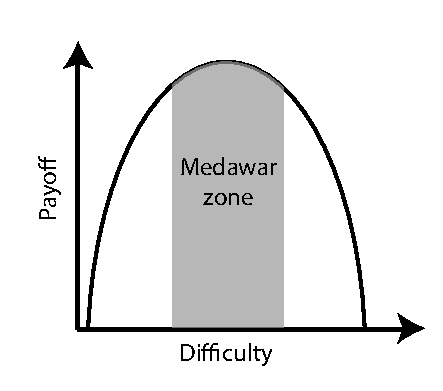
\includegraphics[width = 7cm]{figures/MedawarZone}
\caption{The Medawar zone is an illustration of the sweet spot between too trivial and too difficult questions. The term was coined in \citet{Loehle-guidetoincreased-1990}, in honor of Sir Peter Medawar, who gave a verbal description of this zone in his book `` The Art of the Soluble'' \citep{Medawar-artsoluble-1967}.}
\label{fig: MedawarZone}
\end{center}
\end{figure}

\paragraph{Risks and benefits should balance} In all that, however, you should also make sure that risks and benefits balance - there may be great questions like ``a general cure of cancer'' - it's new, exciting and a valid scientific question. However, if you would try to find an answer in a MSc thesis, you would be set up for failure. Try to find questions that 

\begin{itemize}
\item Don’t test things when the answer is clear
\item To avoid this, don’t pose the question to widely
\item Is a negative result nontrivial? If you can’t show the thing that you expected, is the result still interesting?
\end{itemize}

Great questions\marginnote{If you want to aim really high, you can read the essay ``Ten Simple Rules to Win a Nobel Prize'' by \citep{Roberts-TenSimpleRules-2015}} are also to test a common belief that was not tested before, or question something which was considered established knowledge. 

\section{Validity}

Assuming we have a question of interest and novelty, that seems to be worth pursuing - how can we make sure that we set up a valid scientific procedure to answer it?


A framework that allows us to classify things that can go wrong when we try to apply the scientific method as defined in chapter~\ref{sec: scientific method} is the concept of validity \citep[][]{Shadish-Experimentalandquasi-2002}. The application of these terms is more common in the social science / economics that in natural sciences, but the issues are universal, and for discussing and checking problems I find it useful to have a classification. 

\subsection{Constrcuct validity and bias}

The\marginnote{Construct validity = is what we measure well defined and corresponds to what we mean.} first problem that may appear when we try to test a theory are problems of construct validity. Basically, construct validity means: is what we measure well defined and corresponds to what we mean? Does it correlate with measures it should correlate with (convergent validity)? Is it unrelated to measures it should not correlate with (discriminant validity)?

\paragraph{Construct validity of proxy variables} In "hard sciences" such as physics this is often not so much a concern, but the more we go to complex or social systems, the more likely it is that we measure variables that are proxies for concepts rather than a physical quantity. Examples are "intelligence", "biodiversity", "competition", "light climate". In all these cases, there is probably room for interpretation how to define and measure the concept exactly. It is very advisable to think about his hard, because it can have a strong effect on results. 

\paragraph{Bias} A part of construct validity that is important in either case are potential biases. Biases can appear through instrumental errors, but frequently also through observer bias. More on that in the lecture. 

% TODO \citep{Ransohoff-Biasasthreat-2005}

\subsection{Internal validity}

Internal validity\marginnote{ Internal validity = correlation is not causation} is concerned with the question whether a causal effect can be demonstrated within the experiment / system under study. The basic problem is that correlation does not prove causation. As a an example - if we find that trees have started to grow taller in the last 50 years, and we find that atmospheric carbon dioxide concentration have risen in the same time, we can still not be sure that the CO2 is the causal factor for tree growth. 

Inferences\marginnote{Inferences are said to possess internal validity if a causal relation between two variables is properly demonstrated. } are said to possess internal validity if a causal relation between two variables is properly demonstrated. A more detailed description on this in the \href{https://github.com/florianhartig/ResearchSkills/raw/master/Labs/Statistics/Script/EssentialStatistics.pdf}{accompanying statistics script}, section on experimental design.


\subsection{Statistical validity}

Statistical validity is concerned with the question if an effect has been demonstrated with sufficient statistical (probabilistic) certainty. 

Threats to statistical validity are wrong statistical assumptions, but also explicit and implicit biases through malpractices that are known as multiple testing, researcher’s degrees of freedom, low power,P-value fishing / hacking. A more detailed description on this in the \href{https://github.com/florianhartig/ResearchSkills/raw/master/Labs/Statistics/Script/EssentialStatistics.pdf}{accompanying statistics script}. 

\subsection{External validity}

External validity\marginnote{External validity = do extrapolations hold} asks the question: Does our inference about correlations, or cause-effect relationships hold outside the empirical observations available to use. In other word - can we generalize our study, and if so, to what extent. 

The problem with external validity is that it's hard to demonstrate - if we have measured a plot in a particular location, we cannot be sure a priori how representative it is. In practice, it is a matter of experience and common sense to establish the domain on which your results are valid. Nevertheless, this is a very important task, because it is of course crucial for the results of a study to know how generalization they are. 

\vspace{1cm}

\begin{mdframed}
    
\textbf{Checklist validity}%\\[0.4cm]

Before everything else, make sure the question is well defined. I recommend writing it down to avoid ambiguity. Now, check validity of:

    \begin{itemize}
      \item Construct validity
      \begin{itemize}
        \item Do the variables that you can measure match your question?
        \item What could be sources and extend of errors in your measurement (stochastic, systematic), think also about observer bias etc.
      \end{itemize}
      
      \item Internal validity
      \begin{itemize}
        \item What are potential confound or interacting variables?
        \item How are you planning to control / randomize / measure them? Remember, if you can control is better than measure.
        \item Are you sure about the direction of the causality?
      \end{itemize}     
       
      \item Statistical validity
      \begin{itemize}
        \item How will you analyze your data?
        \item What is the sample size that you need (power)?
        \item Are the problems with the independence of your data? How can you minimize those problems (pseudo-replication, blocked design, ...)
      \end{itemize} 
         
      \item External validity
      \begin{itemize}
        \item What generalization are you planning to make from this study?
        \item What are threads to these generalizations / what could be different in other sites
        \item Is there anything in your design that you can change to allow better generalizations?
      \end{itemize}   
    \end{itemize}

\end{mdframed}


\section{Planning and analysis of experiments} 

Assuming that you have a good question, and that you have checked that you have validity of answering it, how do you perform the measurements and how do you analyze them? A detailed description on all this is in the \href{https://github.com/florianhartig/ResearchSkills/raw/master/Labs/Statistics/Script/EssentialStatistics.pdf}{statistics script} accompanying these lecture notes. I highly recommend reading it. I therefore provide here only bullet points of the things that are absolutely crucial to know. 


\subsection{Planning and experimental design}

If you have considered internal validity, you should already know which variables you need to consider. A more detailed discussion on the choice of variables to maintain internal validity (confounding effects) is in the statistics script. 

As a next step, you will have to decide how you vary the value of those variables (if you have control), and how many observations (replicates) you need. Again, this is discussed in more detail in the statistics script, section on experimental design.

Apart\marginnote{Simulate your analysis before going into the field!} from that, I thin the most important tip for planning an experiment is: play it though! What I mean by that is: simulate how you take your data (for real with a pilot study, or make up some data), analyze it, and see if the results of this analysis correspond, in principle, to what you want to know. In most cases, you will notice that the way you were taking data is not optimal for the statistical analysis, that the analysis you do with your data does not answer what you want to know, or something alike. If you notice that before your experiment, it's easy to fix. If you notice it it afterwards, it isn't. 

\subsection{Analysis}

See chapter "inferential statistics" in the \href{https://github.com/florianhartig/ResearchSkills/raw/master/Labs/Statistics/Script/EssentialStatistics.pdf}{statistics script} accompanying these lecture notes.


\subsection{Visualization}

See chapter "descriptive statistics and visualization" \href{https://github.com/florianhartig/ResearchSkills/raw/master/Labs/Statistics/Script/EssentialStatistics.pdf}{statistics script} accompanying these lecture notes.


\vspace{1cm}
\begin{mdframed}
    
\textbf{Repetition of central concepts in this chapter:} 

\begin{itemize*}
  \item A good scientific question is novel and important, and you should expect to be able to give a valid answer with a acceptable risk of failure
  \item Validity is a classification scheme of problems that can arise when trying to give an answer to a scientific question. See the validity checklist.
  \item You should plan your experiment thoroughly. Part of good planning is that you play the complete process trough before taking the data, including the analysis.
\end{itemize*}

\end{mdframed}



\chapter{Principles and channels of scientific communication}

If you have made a scientific discovery, or at least a little bit of scientific progress, you probably want to let the world know about it. Hence, you need to communicate it.

\section{Principles of communication}

Thinking about communication requires a fundamental change in our attitude - up to now, we have dealt with ourselves, and how to generate knowledge. It was all about finding out the truth. Communication, however, is different. It is not necessarily about saying things right - it is about saying the right things. 

What I mean by that is that the end of communication is not to say things as correct or truthful as they are - the thing that counts is that they are received as correct and truthful as possible by your audience. Good communication therefore requires adjusting to your audience. Before starting to communicate anything, you should therefore ask yourself the following basic questions:


\begin{enumerate}
\item Rule1: Who is my audience?
\item Rule2: What is my main message?
\end{enumerate}

Based on the answer, adjust your words, level of detail, and jokes. There are a few general hints, however, that are always good advice:



\paragraph{Clarity} Science is about getting this right - the main goal of (scientific) communication is therefore clarity and logic. 

\paragraph{KISS} People in science\marginnote{The KISS principle - Keep it short and simple!}, however, are also busy - this means you need to communicate efficiently. Both goals are served well by the KISS principle - Keep it short and simple! However, don't forget Einstein: “as simple as possible, but not simpler”.\footnote{This is also reflected in the following remark by Niels Bohr “Never express yourself more clearly than you are able to think.”}

\paragraph{Jargon} To reach the goals outlined above, Jargon can be a good and a bad thing. It can make communication more efficient, but you have to be careful - this is only the case if you and the recipient have the same jargon. Jargon used in a wrong way is worse than no jargon.


\section{Communication channels}

\subsection{Books and articles}

The most important form of scientific communication is arguably the written word, in form of books and articles. A longer description on how a scientific article is structured is given in the following chapter. 

\subsection{Oral presentations}

The probably second most important channel are presentations. That is, in the perception and attention of many people. Especially young scientists are very concerned with presentations, because they are often grade-relevant, or they feel the social pressure to speak in from of a group. But also for older scientists, presentations are crucial, for example in job interviews. It is therefore important to have some skill in this type of communication \citep[see, e.g. the tips of][]{Kelleher-Tenguidelineseffective-2011}. More material on poster presentations on our \href{https://github.com/florianhartig/ResearchSkills/tree/master/Labs/OralPresentation}{lab on oral presentation}. 

Personally, I think the importance of presentations has decreased. That is not to say that oral presentations are not important - people still give presentations, and you shouldn't suck at it. Often, your job may rely on it. However, it seems to me that, somewhat surprisingly, the age of the internet and new media has moved the scientific debate more strongly back on an old technique - twitter, blogs, forums all work through writing, and these media, as the scientific article, are able to reach a much wider audience than a typical conference talk that is visited by maybe 50 people. 

\subsection{Poster presentation}

Poster presentations are offered on many conferences for participants that don't give a talk. Poster presentations are a great opportunity to meet people and start discussing about your work, but I don't think they rank nearly as high in terms of importance than journal articles. More material on poster presentations on our \href{https://github.com/florianhartig/ResearchSkills/tree/master/Labs/PosterPresentation}{lab on posters}. 


\subsection{Blogs, social media, and such}

Blogs, social media and similar outlets have become more important in recent years. A collection of things that are worth checking out is provided in our \href{https://github.com/florianhartig/ResearchSkills/tree/master/Labs/SocialMedia}{lab on social media}.


\section{Arguments and logical fallacies}

In his article ``Sounder thinking through clearer writing'', \citet{Woodford-Sounderthinkingthrough-1967} cites jargon as one of the key contributors to inefficient communication. He goes further, however, stating that if you communicate without clarity, you will start thinking without clarity yourself, leading to a tendency to draw wrong conclusions. Hence, clear communication is important for you and for others.


A similar case\marginnote{A \href{https://en.wikipedia.org/wiki/List_of_fallacies}{long list of logical fallacies} is provided on Wikipedia} are rhetorical tricks and logical fallacies. There is a long list of archetypical conclusion structures that sound right, but that are typically wrong. Examples of these are

\begin{itemize}
\item False dilemma - example: if we want everything to be completely correct, we can stop doing science!
\item False equivalence - example: no model is completely perfect, therefore there is no difference between using model A and B
\item Strawman - proving an argument wrong that is similar, but not identical to that of the opponent -  example: A: Diversity can increase ecosystem function. B: my opponent suggests that diversity increases ecosystem services. But this is clearly wrong. Imaging a world where we have no HIV virus. Now, if I introduce the virus, we have more diversity. But human well-being is clearly lower!
\end{itemize}

Getting to know these fallacies has many advantages: you will train your logical thinking in general. You will be able to spot these fallacies when used by others. And lastly, you will notice if you use them yourself, avoiding wrong conclusions and sloppy arguments. Therefore, I highly recommend looking at this material!

\vspace{1cm}
\begin{mdframed}
    
\textbf{Repetition of central concepts in this chapter:} 

\begin{itemize*}
  \item Good communication means not saying the right thing, but that your recipient understands what you want him/her to understand - the road to hell is paved with good intentions!
  \item You should know the different communication channels of science. The most important ones are the oral presentation and the scientific paper (next chapter)
  \item Be aware of rhetoric structures and logical fallacies. As a good scientist, you must be able to see through them!
\end{itemize*}

\end{mdframed}



\chapter{Scientific writing}

As already said in the previous chapter: writing is an essential skill for an academic, as for many other professions. \marginnote{The importance of the written word does not seem to change at all in the modern world. The art of writing, similar to public speaking, seems to be one of the stable skills that one can think of.} Despite its central role, however, few master it well. Writing is a subtle art. You can read some advice, but to become a skilled and effective writer requires a long process of observation, practice and reflection: read widely, and think about why some writers appeal to you more. Look critically on your own writing, and think about the things that you can improve. The rest of this section is intended to help you start this journey. 

\section{Some basic writing advice}

\paragraph{Start writing early}Writing\marginnote{Please, follow this point in your thesis - if you don't it leads foreseeable into disaster!} structures your thinking, and you will find flaws in your logic that you didn't see before. "The time to begin writing an article is when you have finished it to your satisfaction. By that time you begin to clearly and logically perceive what it is that you really want to say." (Mark Twain)

\paragraph{Know your audience}Who\marginnote{\citet{Gopen-ScienceOfScientific-1990} state "it matters only whether a large majority of the reading audience accurately perceives what the author had in mind".} is going to read what you write?  You need to adjust your text to the knowledge and background of your audience. 


\paragraph{Know what you want to say, and make a selection!}Sounds\marginnote{"If you don't know where you are going,you'll end up someplace else" (Yogi Berra).} trivial, but in my experience it isn't. Before spending hours on writing the wrong text, try to explain a friend in 5-10 min the essential points of piece, and note the structure. If you fail with this, think again about your story. Also remember: Writing a good paper is not about telling everything you know or have done about a topic -- it is about telling a story and selecting the relevant details. 

\paragraph{Mindset} Make your goal, above all, clarity of thought and expression, and impervious logic of your argument. Read \citet{Woodford-Sounderthinkingthrough-1967}.

\paragraph{Respect conventions}\marginnote{For example, the default scientific article is divided into a title, abstract, introduction, materials and methods, results and discussion. Within these structural elements there are further recognizable patterns. Maintaining this structure makes it easier to understanding of the article's messages \citep{Gopen-ScienceOfScientific-1990,Tischler-Scientificwritingbooklet-1978}} Readers, particularly experienced readers, are familiar with writing conventions expect to find arguments, sections and statements in particular positions and structures. If the writer respects these structural standards the readability is greatly improved. 


\paragraph{Modesty} Think of a scientific text as a piece of craftsmanship, like a chair. What is expected of you is to produce a simple chair that respects the usual standards (e.g. four legs), and that is, above all, solid. You are not expected to add fancy ornamentation that might be used by an ingenious master craftsmen, and produce a entire set of furniture that would suffice to fit out a house. If you could do the later, you would gain admiration and praise, but when trying, you will nearly certainly fail to even produce the very thing you were asked for - a simple, solid chair. Bottomline: stay modest in what you want to achieve, but stay ambitions in how you achieve it!


\paragraph{Style} Writing is difficult. Good writing is incredibly hard. If you think writing is no problem for you, you probably haven't even realized the extent of your writing problems. Read the following section twice!


\section{Style}

Style is personal, and there are many small aspects of style that we cannot cover in a short introduction. However, there are 4 basic properties of style that I find are nearly always missing in undergraduate writing, and then can improve the readability of your text dramatically. 

\subsection{Sentence Structure}

The first is sentence structure. A sentence has two particularly important positions - the  beginning and the end. These two positions have distinct functions \citep{Gopen-ScienceOfScientific-1990,Tischler-Scientificwritingbooklet-1978}.

\paragraph{The topic position} The beginning of a sentence provides us with the context. Typically, we also use it to connect to previous information.

\paragraph{The stress position} The end of the situation provides us with important new information. If it is not clear from the context that we have a logical closure, it also raises the expectation that this new information will be further developed in what is to come. 

Strictly keeping this old-new structure in sentences creates a logical thread, and makes your text easier to read. Reversely, if you bring new information at the beginning of a sentence, it is often hard to understand. An additional bonus of checking your sentence structure is that you are more likely to notice flaws in your logic. I close with a quote from Brian McGill:


\begin{quote}
The battle for good writing is won sentence by sentence! A good sentence is: short, has the subject and verb together, has an active verb, has the points of emphasis at the beginning and end, and moves the reader along from a familiar launch point at the start to the new information at the end. (Brian McGill, on the blog Dynamic Ecology)
\end{quote}


\subsection{Paragraph structure}

A paragraph is supposed to be a logical unit of text. The beginning of a paragraph provides the context. Different to a sentence, the new information should be in the middle of the paragraph. The end of a paragraph is reserved for conclusions (what have we learned in this paragraph). It may also bring up the connection to the next paragraph, e.g. by raising the necessity to look at a particular aspect in more detail. In your writing, make sure your paragraphs have a beginning and a conclusion, and that both are standing out verbally and through simplicity. The latter helps readers that only skimming the text. 

\subsection{Logic}

Your text should be logically flawless. Read again about fallacies. Read about the scientific method and induction. Be careful with the use of logical indicators such as "thus", "hence", "however" - is the implication of this indicators really supported by your argument? More hints in the later section on common mistakes.

\subsection{Clarity}

Keep it simple.\footnote{Mark Twain is famous for his effective writing. A tip from him: "As to the Adjective: when in doubt, strike it out."} More hints in the later section on common mistakes.

\section{The structure of a scientific article}   
% general strucutre

\subsection{A paper from far above}

\paragraph{Structure}Seen far from above, a research paper consists of title, abstract and keywords, and four sections: introduction, methods, results and discussion section. 

\paragraph{Story}A scientific paper, however, is also a story. Many forget that it should be exactly one story. One paper, one story. Be sure you know what your story is. A paper tells the story several times: once in title, once in the abstract, then in the whole paper, and you give additionally summaries of your story in the introduction, and in the discussion and  conclusion.

%hourglass structure
\paragraph{The hourglass} One purpose of telling your story several times is to provide the same information with different levels of details to your reader. The most detailed account is the full paper. Your reader needs to be prepared and led to this level of detail. The idea is that the introduction starts very general, and then becomes more and more specific, until we arrive at the most detailed level at the start of the methods. After the results, we discuss first the immediate results of the paper, and then become wider again, going to implications towards general conclusions. This is known as the hourglass structure. The abstract follows the same structure. 
 
\subsection{Going closer - structural elements in detail}

\paragraph{Title} The title is the first time you tell your story. The main purpose of the title is to inform the reader about the content of the paper. A good and informative title is crucial. Remember that most of your readers will only read the title of the paper.

\paragraph{Abstract}The abstract is the second time you tell your story. Think of the abstract as a mini paper - it has all elements of a paper, but in 300 words. It starts off by setting the scene with a very short and general introduction. This usually links to the second part: Raise the problem. You can emphasize the research question by indicator words like "however".\marginnote{I provide an example later. It may be helpful to copy this as a template into your manuscript when you write your abstract.} Third, you briefly delineate your approach. The fourth subsection serves to state the results. Finally, you present your conclusions and discuss the broader significance.\\

\paragraph{Keywords and other info}Articles usually also have some a list of keywords, usually below the abstract. These terms allow used to be important for indexing purposes in libraries or in the ISI web of knowledge database. Yet, since Google scans whole documents, their importance has decreased. Nevertheless, a good strategy is to choose keywords complementary to title and abstract, e.g. for important technical terms that you did not want to include in the abstract nor title.


\paragraph{Introduction} The\marginnote{The introduction goes from the general to the specific, but not back to the general.} first main section of the article is the introduction. The introduction goes from the general to the specific, but not back to the general. It should consist of four parts, each of which typically has 1-2 paragraphs

\begin{enumerate}\marginnote{To distinguish these parts, you can make use of indicator words: however; problem/ challenge; here we used; we applied; we asked; we tested.}
\item Introduce the topic. Lay out relevance and what has been done before. Here you usually cite a lot of literature showing that you know the current state of knowledge concerning the topic of your study.
\item Explain the problem, i.e. the gap of knowledge. You should demonstrate novelty as well as relevance.
\item Explain your approach: What are your methods; what are the data you used?
\item List your specific research questions. This subsection does not need to be clearly separated from the approach subsection. It should however, provide a link to the result sections by outlining the work flow of the analysis.
\end{enumerate}

\paragraph{Methods} The methods section explains the methods. It needs to be short, because paper space is limited. Technical details (Software version, etc.) are nowadays often moved into an online supplementary. Nevertheless, the methods should provide sufficient information to repeat the study in principle.\marginnote{Keyword is repdoucibility.}. The method section is often divided in subsections such as study area, data, statistical analysis/ model, analysis, etc. Another helpful tip is to add figures. One further tips: problems with your methods are not discussed here, but in the conclusions. 


\paragraph{Results} The results present the results of the analysis, as clear as possible. They state only facts, but do not interpret them (unless the interpretation is obvious). The latter is the job of the discussion. The presentation of the results should follow the questions in the introduction. If you have three questions, you would usually have three subsections. 

\paragraph{Discussion/ Conclusion} The discussion summarizes the findings of the paper, and discusses it's implications and broader relevance. It moves from the specifics of your particular study to back to the general level. 


\begin{enumerate}\marginnote{The discussion moves from the the specific to the general.}
\item Questions and main findings in short
\item Comparison to other findings
\item Limitations and further research
\item Conclusions, and broader impacts for science and society
\end{enumerate}

The first part has the function of providing a lazy reader with the question and directly the findings of the study. The second part will discuss how these findings fit to previous research, if knowledge needs to be updated and so on. \marginnote{Only discuss the limitations that question/limit the credibility of your results.} You will then typically proceed to limitations of your approach. The goal is to establish the domain under which your results are valid; do not question your approach in general, or list everything that could have been done as well. The final paragraph is very important - it provides your conclusions and outlook on the subject. 

\section{Showcase: A commented paper}


\begin{center}
	\huge{Fancy analysis supports hypothesis\marginnote{Try to capture the questions, methods, and main results of your study in the title, if possible} X as the main cause high species diversity in tropical forests} \\ 
	\vspace{0.3em}
	\large{Florian Hartig and Severin Hauenstein}\\
	\vspace{0.3em}
	\small{\textit{Department of Biometry and Environmental System Analysis, University of Freiburg, 79106 Freiburg, Germany}}\\
	\vspace{1em}
	\large{\today}\\
	\vspace{2em}
	\textbf{Abstract}\\ \marginnote{Remember: the abstract is a mini-paper}
\end{center}
\begin{quote}
Tropical forests are some of the most species-rich ecosystems\marginnote{First words set the scene} of the world.
The reason for this, \textbf{however}, is still widely debated\marginnote{Raise the problem. Indicator word: however}. Hypotheses range from processes related to productivity over environmental stability to the historical changes in geography.
\textbf{Here}\marginnote{Introduce your approach. Indicator word: here}, we contrasted these different hypotheses by using data from ... together with ... (fancy new method).
\textbf{We find that}\marginnote{State your results. Indicator word: We find, our results are ...} hypothesis X seems to be significantly better supported by our data
than all alternatives we tested. Specifically ... 
\textbf{In conclusion}\marginnote{Give your conclusions and discuss wider significance. Indicator word: in conclusion, ...}, our study supports the hypothesis that species diversity in the
tropics is mainly driven by higher productivity. These results challenge some long held
ideas about geographical stability being the main reason for global diversity
patterns. They also have important practical applications for mitigation of climate
change, as ...\\[0.3cm]
\noindent\textbf{Keywords:}\marginnote{Keywords for indexing purposes.} Biodiversity -- Primary production -- Floristic structure ...\\
\end{quote}

\noindent\textbf{Introduction}\\
Tropical forests\marginnote{Introduce the topic. Explain relevance. Remember intro should mirror the abstract, one sentence in the abstract = one paragraph intro} are some of the most species-rich ecosystems. According to XY (19XX) tropical forests make up fo x \% of the planet's biodiversity.\\
...

The\marginnote{Introduce the problem (1-2 paragraphs)} reason for high diversity in the tropics is still widely debated. Historically, it was though [...]. More recently, however, the view has emerged that [...] (e.g. ABC, 19XX; D\&E, 20XX; FG, 20XX). Up to now, none of these theories has been tested to an extend that it could be excluded as a potential explanation for the high tropical biodiversity\\
...

While the hypotheses described earlier cannot be tested directly,\marginnote{Introduce your approach ... could also be, as here, by explaining a new option to address the problem} a possible route would be to conduct and indirect test via the method of ABC (19XX). This method has originally been developed for X, but it should be able to distinguish among Y and Z. To our knowledge, no such test has been performed yet.\marginnote{Demonstrate novelty}
\\
...

We\marginnote{Approach, now more specific} therefore applied X to compare the the support for the main hypotheses published by ABC (19XX), D\&E (20XX), FG (20XX). For the latter we used X data provided by XYZ (2014). We first test X in order to find the difference in Y. As an alternative approach we choose to look at Z for the purpose of XY.\\
... 

We\marginnote{Questions at the end of the intro should mirror sections in the results and discussion in the conclusion.} ask the following questions:

\begin{enumerate}
\item Which of the three hypothesis receives most support from the data
\item Question 2
\item Question 3
\end{enumerate}

\noindent\textbf{Methods}\\

This section is typically divided into

\begin{enumerate}
\item Study area
\item Experimental procedure
\item Statistical analysis
\end{enumerate}

\noindent\textbf{Results}\\

The presentation of the results should follow the questions at the end of the introduction. If you had three questions, you would typically make three subsections.

\noindent\textbf{Discussion}\\
In this study\marginnote{Summarize main conclusions}, we used method X to test whether prevalence of A is associated to factor B. Our main result is that there is a significant correlation of B with A. This correlation, however, was only found when factor C was also present.

Our\marginnote{Discuss relation to other studies and scientific implications} findings support earlier findings of (X, 2005) and (Y, 2002) who also found a positive correlation between A and B. The fact that this correlation was only present in samples under conditions C may also explain previous opposite results such as (ZZ, 2006,2008), as neither of these previous studies controlled for C. The reason for this positive association and the fact that it is affected by C is still unknown. We speculate that mechanism R could be a reason for this. This idea is given further support by the observation that the correlation between A and B is affected by C. Such an effect would be expected if R is really the cause of this Correlation, as R is dependent on C (XAY, 1968).

A\marginnote{Discuss limitations and scope of the conclusions (see external validity). Limitations is not everything that could also have been done.} limitation of our study is the geographical limitation of our data. As we could only retrieve data from the neotropics, but not from Africa or Asia, we can currently not say if our results will hold globally.

A\marginnote{Limitations are often connected to ideas for further reasearch} further issue is the possibility that niche conservatism contributes to the observed signal. Currently, we lack sufficient genetic data to obtain high-resolution phylogenies that could be used to test for this effect. However, as these data become increasingly available, future studies should include phylogenetic information to exclude this possibility. 

In conclusion\marginnote{End with conclusions and wider importance for science and society}, the results of our study supports the idea that X is the main mechanism for the high diversity in the tropics. This has important implications for global biodiversity conservation [...], as well as for our understanding of the maintenance of diversity.\marginnote{Some people end with further research here. I find this a bit weak and prefer to deal with this topic in the earlier paragraphs.}

\section{A list of common writing problems}


\begin{enumerate}[(A)]


\item Strategic writing problems
\begin{enumerate}
	\item Do not make statements that are unnecessary for your argument, but could be questioned. 
	Example: "The two most classic games to simulate the behavior of animals are the Hawk-Dove game and the Prisoner's Dilemma." $\rightarrow$ Others might disagree. Is it really important to be so definite here? Why not say: "Two classic games..."?
	\item Passive/ Active: See the comments in the lecture notes on scientific writing. In general you should write in an active voice, unless  1) Sentence structure C3 takes precedence, or 2) the thing you talk about is impersonal, was done by another person. More details in the lecture notes. In particular, opinions of your own \textsc{should} be active.
	\item Be definite - remember Yoda: There is no try, do it. Phrases like: "we attempted to find whether there is" or "this study aims at" sound weak and defensive. Write "we studied whether ...". Also: "to the best of our knowledge ... " This is a borderline case. You will see this expression in scientific articles, and it's OK to use it. However, it does seem insecure. Better to indicate that you made some effort to find out together with such an expression. 	
	
 

\end{enumerate}

\item Logical problems
\begin{enumerate}
	\item The stated implication does not follow the argument logically. Example: "Because both models follow different pay-off schemes, it is important to know how a simulation model reacts to different settings." $\rightarrow$ Unclear why it is important to know how simulation reacts to different settings if two models are different.
	\item "Micrologic": Logical indicators such as "thus", "hence", "however", "nevertheless" have a clear and distinct meaning. "thus", "hence" indicate an implication. "however", "nevertheless" indicate contradicting statements or evidence to the previous proposition.
\end{enumerate}


\item Style
\begin{enumerate}
	\item Drop redundant words: Any of the following \textbf{words} can be erased: "\textbf{a total of} n subjects", "the simulations were run with the \textbf{exact} same parameter set as before"
	\item Pompous/ pontificating style: If something can be said in simple words, it should be said in simple words, i.e. if the only purpose of a sentence is to "sound scientific", it should not be said at all. Examples: The data \textbf{featured/comprised} a pixel size of 10 (had). We utilized (use).\footnote{Styleguides advice against complicated words such as utilize if there are simpler equivalent alternatives, although others have argued that there is a different between use and utilize - but could you name it? See discussion here \href{http://en.wiktionary.org/wiki/utilise}{here}.} We used the model in an integrated framework to facilitate a holistic forecast" (predicting from the model). Tip: Read \citet{Woodford-Sounderthinkingthrough-1967}.
	\item Topic position/ Stress position not properly occupied: The first part of a sentence should give the context. The last part of the sentence should provide the crucial new information, and should relate to what is further discussed. Tip: Read \citet{Gopen-ScienceOfScientific-1990}.
	\item A paragraph structures the text into topical units. Use them! Each paragraph should introduce its topic in the beginning, and ideally lead to some conclusion or summary at the end. 
	\item Unnecessary adjectives. Mark Twain: "As to the adjective: when in doubt, strike it out." Especially adjectives such as "very", "particularly" are often not necessary. Applies also to larger constructs such as "Evolutionary Game Theory \uline{is an important tool to} investigate(s) ..." -- if you erase the underlined text, the sentence remains fine.
	\item Unclear/ ambiguous expressions: Write as clear and as informative as possible. Avoid ambiguous words like "tends to", "mostly" etc. if you can make a definite statement. Example: "the frequency of cooperators always tends to be zero"  $\rightarrow$ What does that mean? 1) It was always zero or 2) It was zero in 95 \% of the cases or 3) something else.
\end{enumerate}

\item Grammar and spelling

\begin{enumerate}
	\item English commas have different rules than in German and other languages \url{http://www.grammarbook.com/punctuation/commas.asp}
	\item Wrong use of \textbf{which and that} Let's say that we have 10 samples. Compare the two sentences: 1) the samples, which were expose to radiation the day before, were analysed. 2) The samples that were exposed to radiation the day before were analyzed. The important difference is that 1) says all samples were exposed to radiation and then analysed, while 2) implies that not all samples were exposed to radiation, and only those that were were analysed. 1) is called a non-restrictive clause, and 2) is called a restrictive clause. "that" always implies a restrictive meaning. Additional confusion, however, is created by the fact that "which" can in fact be used for both, with a minor modification: if you want to use which restrictive, you have to write 3) The samples which were exposed to radiation the day before were analyzed. Notice that there is a tiny difference to 1) - there is no comma before which. This is the only indicator that allows us to know whether the restrictive or the non-restrictive meaning is implied. Many people are not aware of this difference though. In prose, the distinction may matter little, but for science, my opinion is that clarity goes before style, and I therefore recommend to strictly stay with 1) which for non-restrictive and 2) that for the restrictive meaning.
\end{enumerate}



\end{enumerate}


\section{Examples}

In the following, I highlighted \uline{redundant words} and other problems

\begin{itemize}

\item A \uline{subsequent} ANOVA \uline{analysis} \textbf{enabled a quantification of} the impacts of the varied factors (quantified)

\item There are \uline{a number of records} in the literature \uline{focusing on comparisons} between \uline{sets of }modeling approaches while predicting biomass at plot scale (A number of previous studies has compared modeling approaches to predict biomass at the plot scale)

\item \uline{As such}, the \uline{explicit} findings of our two experiments showed that \uline{a total of} 9 samples ... 

\end{itemize}


\vspace{1cm}
\begin{mdframed}
    
\textbf{Repetition of central concepts in this chapter:} 

\begin{itemize*}
  \item A sentence starts with the context and ends with the new info
  \item A paragraph starts with the topic, discusses the topics, and ends with a summary and connection to the next point
  \item Write with clarity and logic
  \item Follow the standard structure. No experiments!
  \item Read through the list of common writing problems!
\end{itemize*}

\end{mdframed}

\chapter{A working scientists}

We have covered by now the primary scientific process from deciding on a scientific question, generating valid data and conclusions, and communicating those in writing or through other channels. What remains are the aspects that relate to science is also a human and professional endeavor. The purpose of this chapter is to give a very fast overview on questions such as professional norms and ethics, as well as career options and the working life of scientist.

\section{Professional ethics and good scientific practice}

The term "good scientific practice" encompass the accepted rules and norms of the field. They structure around subjects such as 

\begin{itemize}
\item Honesty in data generation and the presentation of results (don't falsify data)
\item Honesty in attribution (authorship, plagiarism, etc)
\item Standards of professional work (data storage, lab notebook, ...)
\item Contribution to the scientific society (share data, contribute to common goods such as reviewing)
\end{itemize}

Many\marginnote{The rules of the German Science Foundation (DFG) are available \href{http://www.dfg.de/en/research_funding/principles_dfg_funding/good_scientific_practice/}{here}. Other guidelines for good scientific practice are available \href{https://github.com/florianhartig/ResearchSkills/blob/master/Labs/AcademicSoftSkills/codesOfConduct.md}{here}}
 universities, institutes, and funding organizations have explicit rules of good scientific practice \citet[e.g.][]{Forschungsgemeinschaft-RulesGoodScientific-2013}. The following paragraphs give a fast overview about the most important topics:


\paragraph{Fabrication and falsification} You must not do this!

\paragraph{Misrepresentation of results} You\marginnote{Misrepresentation would be knowingly using wrong statistics, or claiming something you haven't shown} must not do this either!

\paragraph{Documentation and organization} There\marginnote{Simple things like having a good folder structure for each project help a lot. Have a look at our lab on \href{https://github.com/florianhartig/ResearchSkills/tree/master/Labs/ProjectOrganization}{project organization}} is no clear legal rule about how long data, documentation and samples have to be stored, but most funding organizations recommend a 10yr period. Depending on the discipline, not having a lab notebook or storing your data would be considered something between a sloppy behavior and a sever and highly suspicious misconduct (many ecological researchers, for example, have very sloppy or no lab/field notebooks. In medical research, lab notebooks are taken extremely serious.)\marginnote{When working with code, specially collaboratively, there is no way around using a version control system. See our lap on version control \href{https://github.com/florianhartig/ResearchSkills/tree/master/Labs/VersionControl}{here}}

\paragraph{Attribution and authorship} A common problem is also the attrition of work, i.e. authorship and plagiarism. You know you should not copy text from others (plagiarism). You also should not copy text from yourself and publish it again to appear to be more productive (self-plagiarism). Authorship is a difficult issue. More on that in the lecture. 

%\section{Social aspects}

%\subsection{Collaborations and teams}

%\subsection{Conflicts}

%\subsection{Intercultural issues}


%\section{Science as a career}

%\marginnote{Read the special feature in Nature on the \href{http://www.nature.com/news/specials/phdfuture/index.html}{future of the PhD}}


\vspace{1cm}
\begin{mdframed}
    
\textbf{Repetition of central concepts in this chapter:} 

\begin{itemize*}
  \item Read and follow the rules of good scientific practice 
\end{itemize*}

\end{mdframed}


\bibliographystyle{/Users/Florian/Home/Bibliography/Databases/bibstyles/elsart-harv-hyperlinks}
\bibliography{/Users/Florian/Home/Bibliography/Databases/flo}

\end{document}
